% !TEX root = ../../thesis.tex


% \cleardoublepage
% \newpage
% \thispagestyle{plain}
% \mbox{}
\includepdf{/Users/matthieulapeyre/Documents/phd_thesis/media/thebeast.pdf}


\chapter{Robot morphology: some facinating work} % (fold)

\textbf{Object}: In this chapter, we will present a review of different research which has already explored the role of the mophology


\textbf{Conclusion}: The body can definitely take in charge a part of the complexity. And we need to continue studying it by EXPERIMENTATIONS. Even if simulator can be complementary.
% chapter exploration_of_the_morphology_role (end)


% Photo Yves Gellie
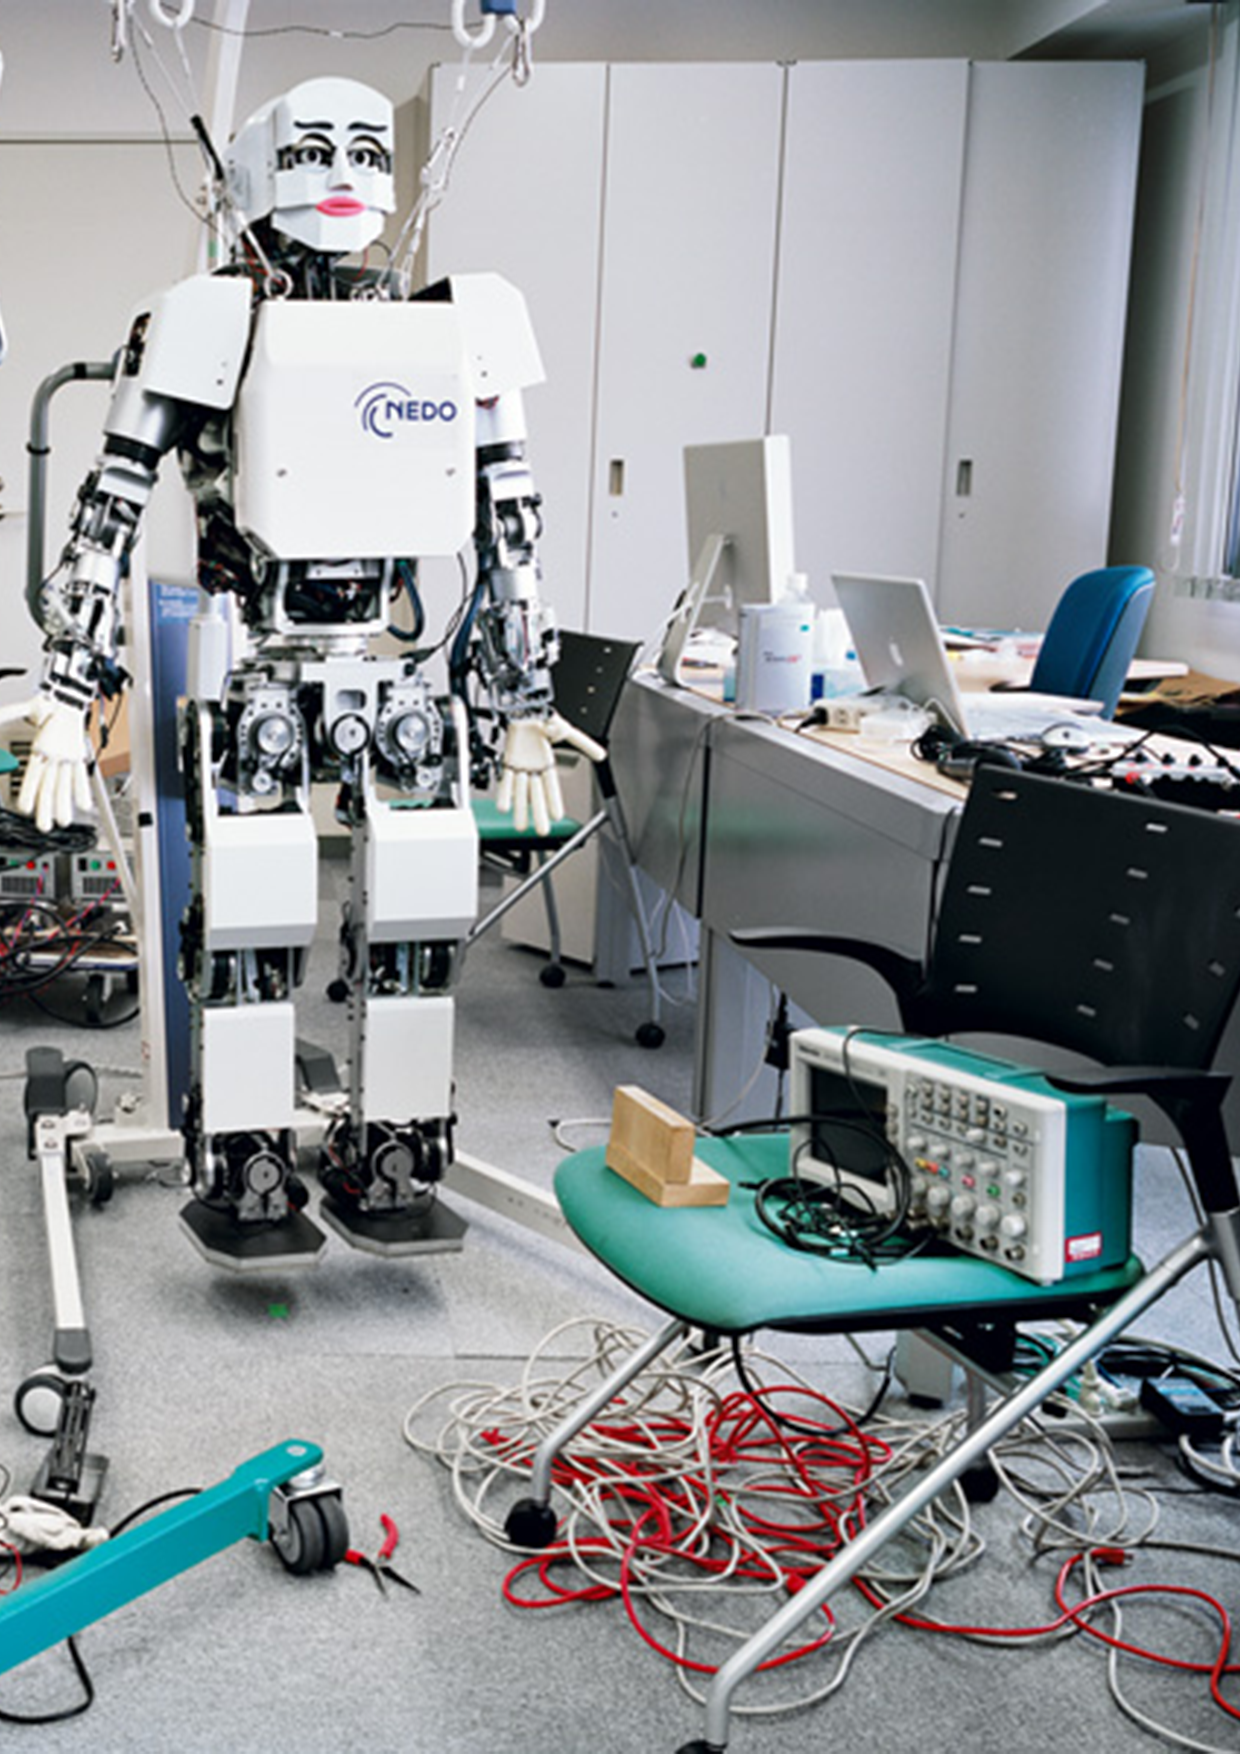
\includepdf{/Users/matthieulapeyre/Documents/phd_thesis/media/robot_setup.pdf}
\chapter{Current robotic platforms} % (fold)

\textbf{object}: Review of the robot, in particular biped.


\textbf{Conclusion}: There is no adapted or replicable platform. We need to create one.



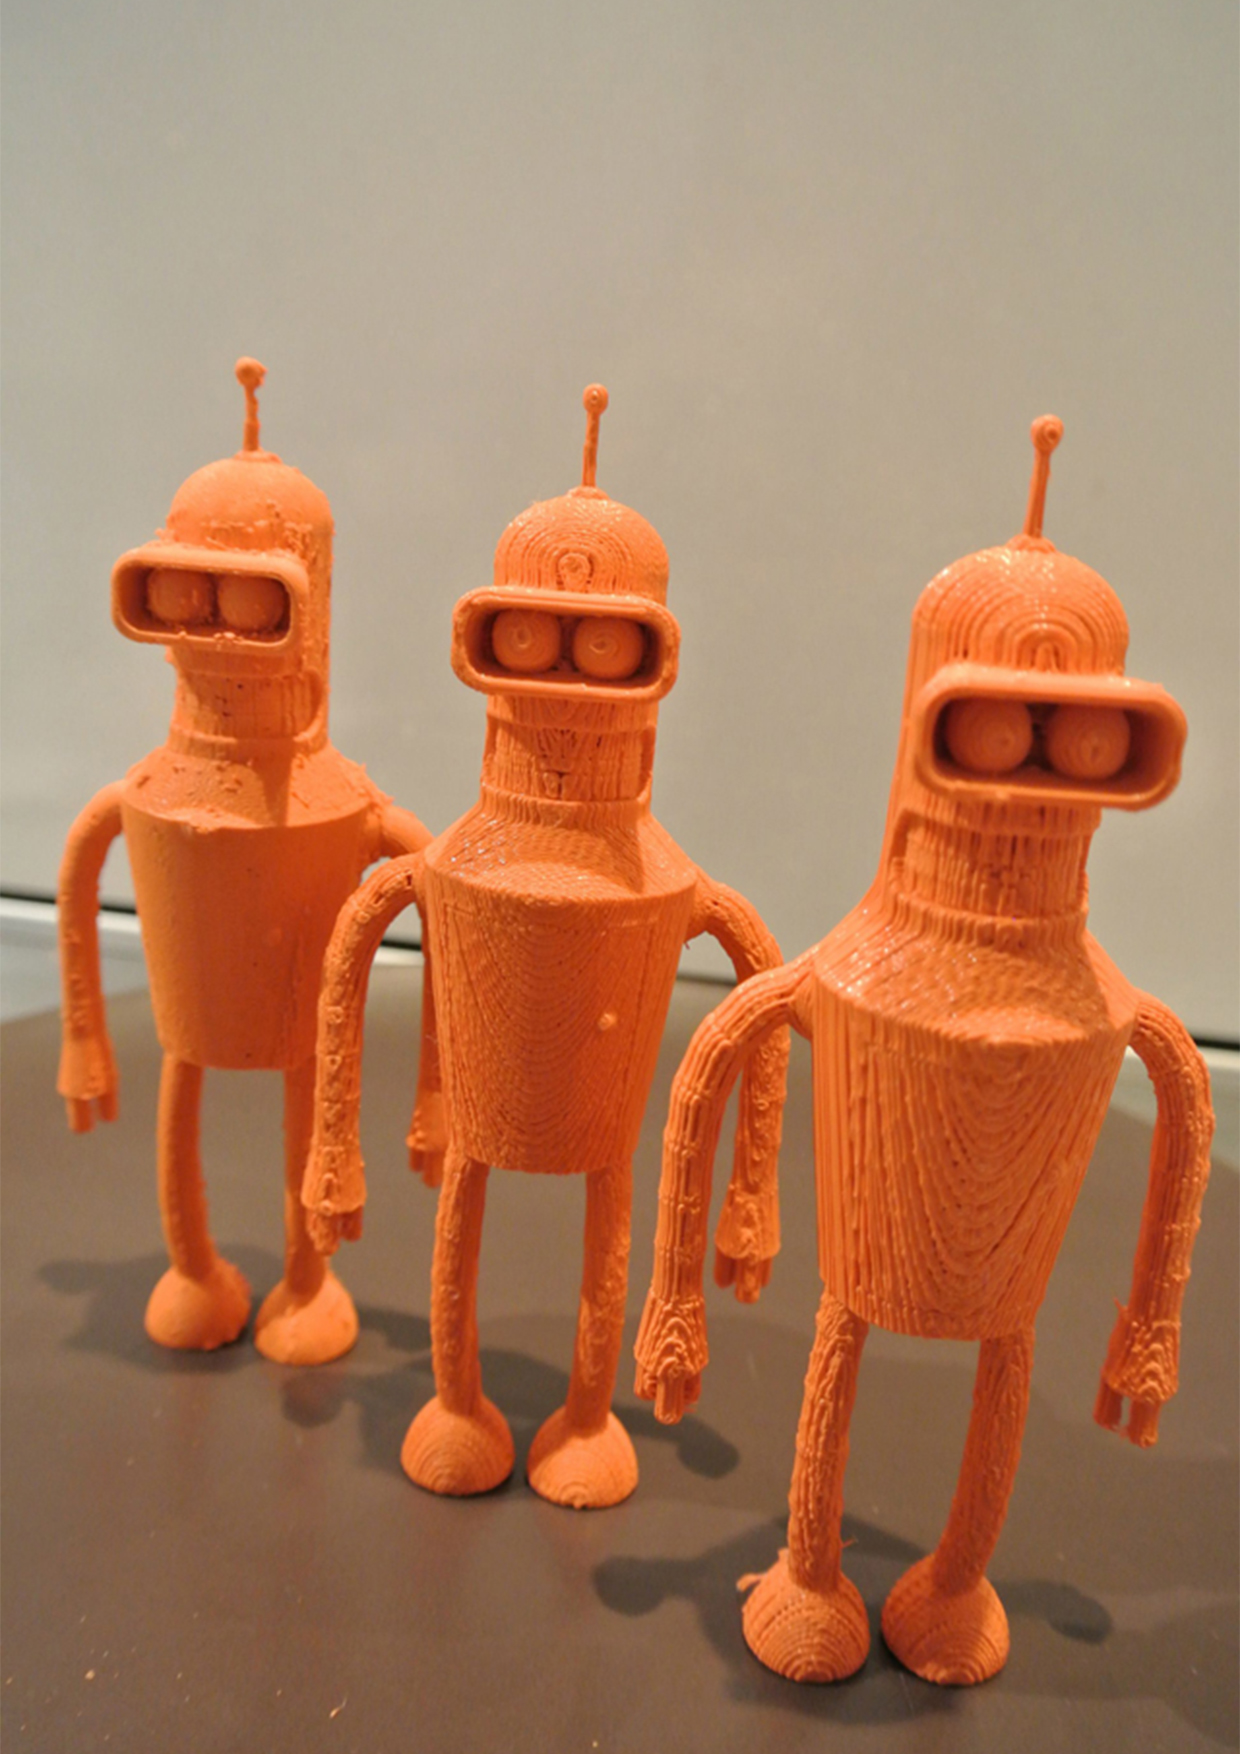
\includepdf{/Users/matthieulapeyre/Documents/phd_thesis/media/3DprintedBlender.pdf}
\chapter{The open hardware and 3D printing revolution} % (fold)

http://alternatives.blog.lemonde.fr/2014/04/06/ces-projets-open-source-qui-changent-le-monde/